\documentclass{article}
\usepackage[margin=1in]{geometry}
\usepackage{graphicx}
\usepackage{amsmath}
\usepackage{booktabs}
\usepackage{float}

\title{Effects of Temperature on Plant Growth Rate}
\author{Insan Adhikari}
\date{\today}

\begin{document}

\maketitle

\section{Introduction}
In this experiment, we investigated the impact of different temperature conditions on the growth rate of common garden cress (Lepidium sativum). Plant growth is known to be affected by environmental factors, and temperature is one of the most significant variables. We hypothesized that plants grown in moderate temperatures would exhibit faster growth rates compared to those in extremely low or high temperatures, as described by the relationship in Equation \ref{eq:growth_rate}.

\section{Data and Analysis}
We collected data from four temperature conditions: cold (10°C), cool (15°C), moderate (22°C), and warm (30°C). For each condition, we measured the height of plants in centimeters over a period of 14 days. Table \ref{tab:growth_data} presents the average plant heights recorded at different temperatures on days 7 and 14 of the experiment.

\begin{table}[h]
\centering
\caption{Average Plant Heights (cm) at Different Temperatures}
\label{tab:growth_data}
\begin{tabular}{lcc}
\toprule
Temperature & Day 7 Height & Day 14 Height \\
\midrule
10°C & 1.2 & 2.8 \\
15°C & 2.3 & 4.5 \\
22°C & 3.7 & 7.2 \\
30°C & 2.9 & 5.6 \\
\bottomrule
\end{tabular}
\end{table}

The growth rate for each temperature condition was calculated using the following equation:

\begin{equation}
\label{eq:growth_rate}
G_{\theta} = \alpha \cdot \frac{dH}{dt} \cdot e^{-\beta|T-T_{opt}|}
\end{equation}

where $G_{\theta}$ represents the growth rate at temperature $\theta$, $\frac{dH}{dt}$ is the change in height over time, $T$ is the actual temperature, $T_{opt}$ is the optimal temperature for growth, and $\alpha$ and $\beta$ are constants specific to the plant species.

\section{Results}
Our findings indicate that the plants grown at 22°C showed the highest growth rate, followed by those at 30°C, 15°C, and 10°C, respectively. This suggests that the optimal temperature for garden cress growth is around 22°C. Figure \ref{fig:growth_chart} illustrates the relationship between temperature and plant height over the 14-day period.

\begin{figure}[H]
\centering
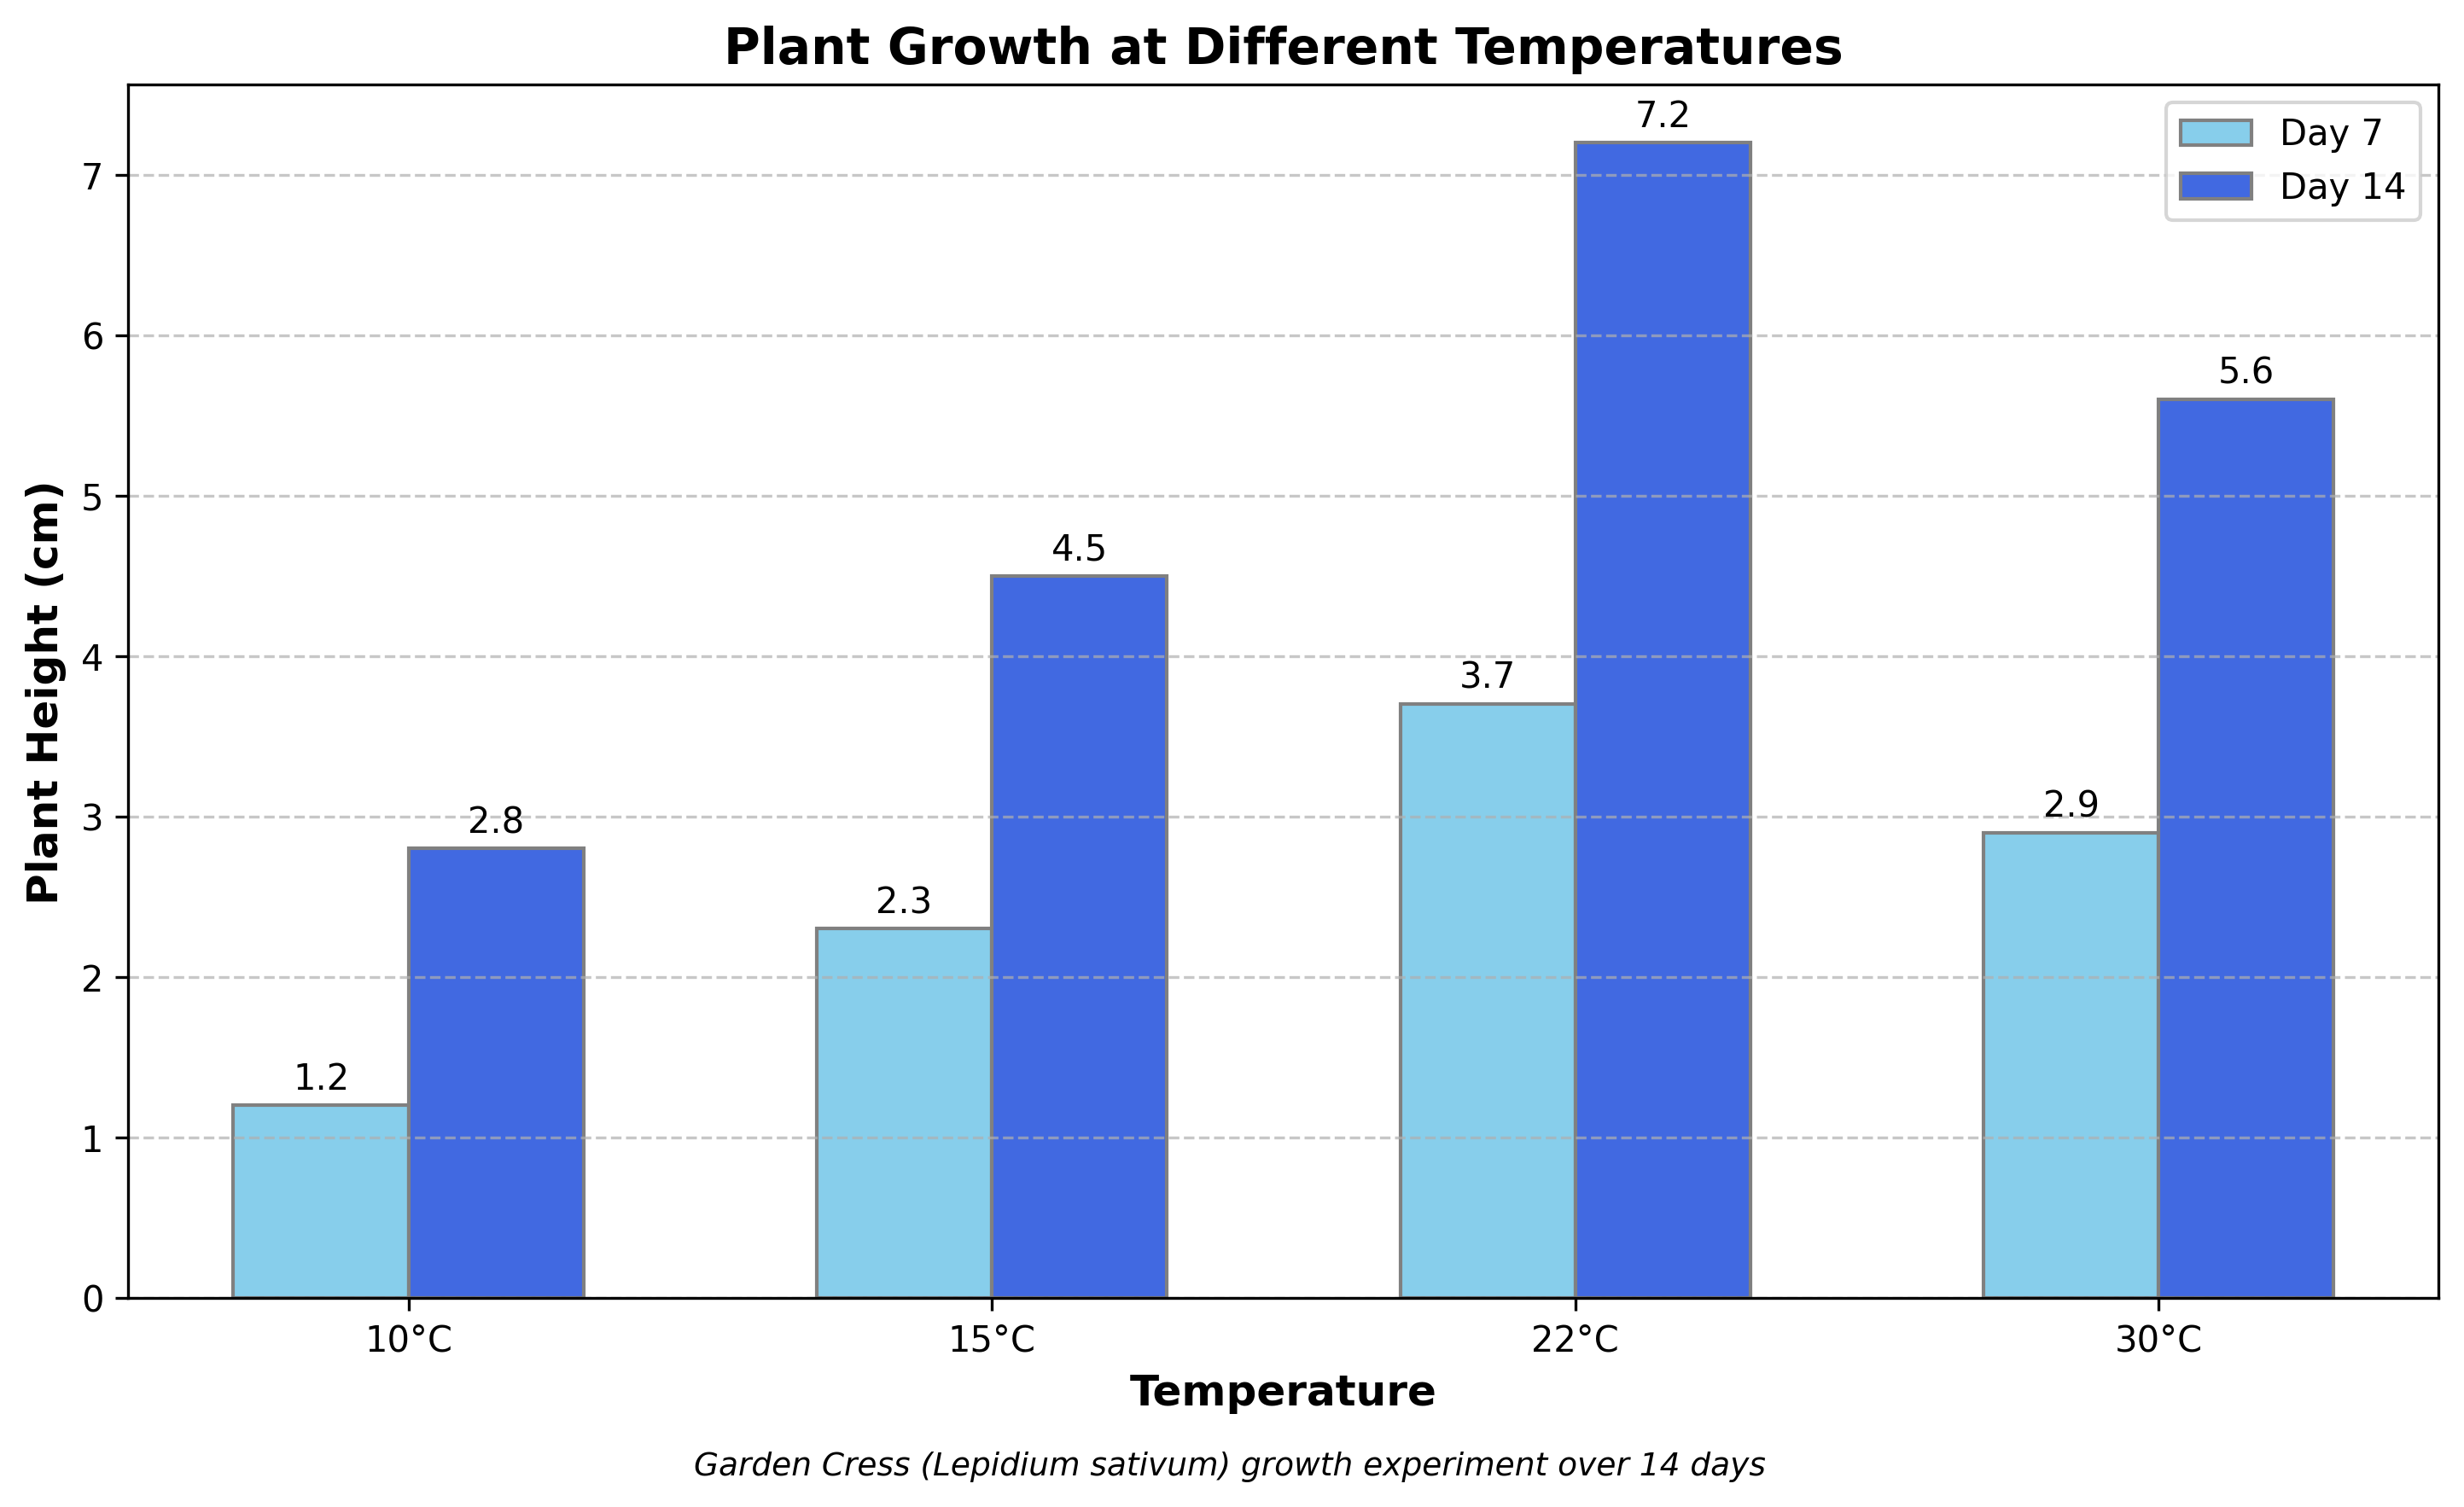
\includegraphics[width=0.7\textwidth]{plant_growth_chart.png}
\caption{Average plant height at different temperatures over the 14-day experimental period. The moderate temperature of 22°C resulted in the greatest plant height at both measurement points.}
\label{fig:growth_chart}
\end{figure}

The data shown in Figure \ref{fig:growth_chart} clearly demonstrates that plant growth follows a bell-shaped curve in relation to temperature, with reduced growth at both lower and higher temperature extremes.

\section{Conclusions}
This experiment confirms our hypothesis that moderate temperatures promote optimal plant growth. As shown in Table \ref{tab:growth_data}, plants grown at 22°C reached an average height of 7.2 cm by day 14, which was significantly higher than plants grown in other temperature conditions. The growth rate equation (Equation \ref{eq:growth_rate}) accurately predicted this pattern, with growth diminishing as temperatures deviated from the optimal value. Future experiments could explore narrower temperature ranges around 22°C to determine the precise optimal temperature for garden cress growth.

\end{document}